% LORE-KV architecture figure (Algorithm 1). Build: scripts/make_readme_assets.py
% (compiles with tectonic or pdflatex, then writes assets/lorekv_architecture.{svg,png}).
\documentclass[tikz,border=6pt]{standalone}
\usepackage[default]{sourcesanspro}
\usepackage{amsmath,amssymb,bm}
\usetikzlibrary{positioning,calc,arrows.meta,decorations.pathreplacing,backgrounds,fit}

% ---------------------------------------------------------------- palette
\definecolor{ink}{HTML}{14161A}
\definecolor{ink2}{HTML}{52514E}
\definecolor{muted}{HTML}{A3A29C}
\definecolor{rule}{HTML}{E2E1DC}
\definecolor{card}{HTML}{FFFFFF}
\definecolor{surface}{HTML}{F7F7F4}
\definecolor{lblue}{HTML}{2A78D6}
\definecolor{lbluebg}{HTML}{E8F1FC}
\definecolor{lorange}{HTML}{EB6834}
\definecolor{loranbg}{HTML}{FDEEE7}
\definecolor{laqua}{HTML}{1BAF7A}
\definecolor{lviolet}{HTML}{6250D6}

\tikzset{
  card/.style={draw=rule, line width=0.6pt, fill=card, rounded corners=5pt,
               minimum width=4.05cm, minimum height=4.15cm, anchor=north},
  tok/.style={draw=none, rounded corners=0.8pt, minimum width=0.16cm, minimum height=0.36cm, inner sep=0},
  flow/.style={-{Latex[length=2.2mm,width=1.8mm]}, line width=0.9pt, draw=ink2},
  num/.style={circle, fill=#1, text=white, font=\bfseries\scriptsize, inner sep=0pt, minimum size=4.2mm},
  ttl/.style={font=\bfseries\normalsize, text=ink, align=center},
  body/.style={font=\footnotesize, text=ink2, align=center, text width=3.9cm, execute at begin node={\hyphenpenalty=10000\exhyphenpenalty=10000}},
}

% ---------------------------------------------------------------- icons
% token strip: #1 = list of fill colors
\newcommand{\tokenstrip}[2]{% #1 origin, #2 colors
  \foreach \c [count=\i from 0] in {#2} {
    \node[tok, fill=\c] at ($(#1)+(\i*0.2,0)$) {};
  }}

\begin{document}
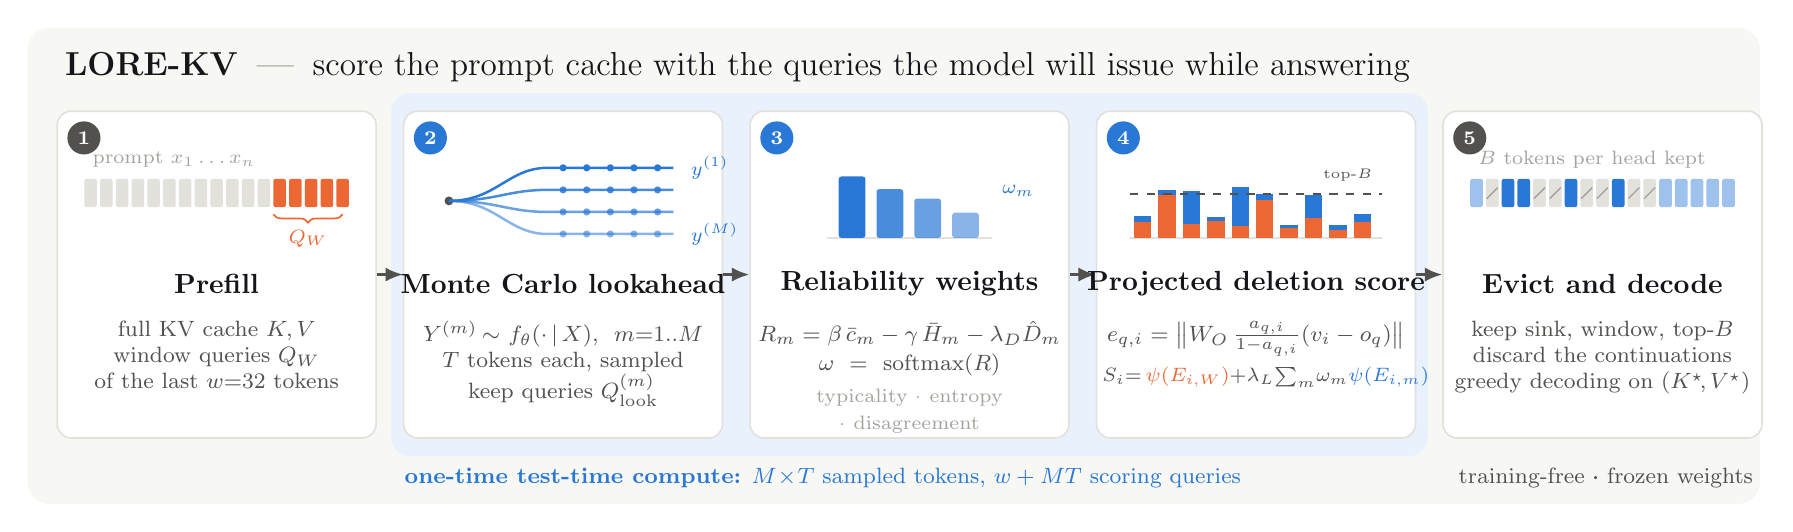
\begin{tikzpicture}[x=1cm,y=1cm, font=\small]

% background
\begin{scope}[on background layer]
  \fill[surface, rounded corners=8pt] (-0.35,0.95) rectangle (21.65,-5.1);
\end{scope}

% title
\node[anchor=west, font=\bfseries\large, text=ink] at (0,0.45)
  {LORE-KV \,\textcolor{muted}{|}\, \mdseries score the prompt cache with the queries the model will issue while answering};

% cards
\foreach \k/\x in {1/2.05,2/6.45,3/10.85,4/15.25,5/19.65} {
  \node[card] (c\k) at (\x,-0.1) {};
}
% one-time lookahead bracket (stages 2-4)
\begin{scope}[on background layer]
  \fill[lbluebg, rounded corners=7pt] ($(c2.north west)+(-0.15,0.22)$) rectangle ($(c4.south east)+(0.15,-0.22)$);
\end{scope}
\node[font=\scriptsize\bfseries, text=lblue, anchor=south] at ($(c3.north)+(0,0.24)$) {};

% arrows between cards
\foreach \a/\b in {1/2,2/3,3/4,4/5} { \draw[flow] (c\a.east) -- (c\b.west); }

% ------------------------------------------------ stage 1: prefill
\node[num=ink2] at ($(c1.north west)+(0.35,-0.35)$) {1};
\tokenstrip{$(c1.north)+(-1.6,-1.05)$}{rule,rule,rule,rule,rule,rule,rule,rule,rule,rule,rule,rule,lorange,lorange,lorange,lorange,lorange}
\draw[decorate,decoration={brace,mirror,amplitude=3pt}, draw=lorange, line width=0.6pt]
  ($(c1.north)+(0.72,-1.32)$) -- ($(c1.north)+(1.6,-1.32)$) node[midway,below=2pt,font=\scriptsize,text=lorange]{$Q_W$};
\node[font=\scriptsize, text=muted, anchor=west] at ($(c1.north)+(-1.7,-0.62)$) {prompt $x_1\dots x_n$};
\node[ttl] at ($(c1.north)+(0,-2.2)$) {Prefill};
\node[body, anchor=north] at ($(c1.north)+(0,-2.55)$)
  {full KV cache $K, V$\\window queries $Q_W$\\of the last $w{=}32$ tokens};

% ------------------------------------------------ stage 2: Monte Carlo lookahead
\node[num=lblue] at ($(c2.north west)+(0.35,-0.35)$) {2};
\coordinate (r) at ($(c2.north)+(-1.45,-1.15)$);
\fill[ink2] (r) circle (1.6pt);
\foreach \dy/\op in {0.42/1,0.14/0.85,-0.14/0.7,-0.42/0.55} {
  \draw[lblue, line width=0.9pt, opacity=\op] (r) .. controls +(0.6,0) and +(-0.5,0) .. ($(r)+(1.25,\dy)$) -- ($(r)+(2.85,\dy)$);
  \foreach \t in {1.45,1.75,2.05,2.35,2.65} { \fill[lblue, opacity=\op] ($(r)+(\t,\dy)$) circle (1.3pt); }
}
\node[font=\scriptsize, text=lblue, anchor=west] at ($(r)+(2.95,0.42)$) {$y^{(1)}$};
\node[font=\scriptsize, text=lblue, anchor=west] at ($(r)+(2.95,-0.42)$) {$y^{(M)}$};
\node[ttl] at ($(c2.north)+(0,-2.2)$) {Monte Carlo lookahead};
\node[body, anchor=north] at ($(c2.north)+(0,-2.55)$)
  {$Y^{(m)}\!\sim f_\theta(\cdot\,|\,X)$, \ $m{=}1..M$\\$T$ tokens each, sampled\\keep queries $Q^{(m)}_{\text{look}}$};

% ------------------------------------------------ stage 3: reliability weights
\node[num=lblue] at ($(c3.north west)+(0.35,-0.35)$) {3};
\coordinate (b) at ($(c3.north)+(-0.9,-1.62)$);
\draw[rule, line width=0.6pt] ($(b)+(-0.15,0)$) -- ($(b)+(1.95,0)$);
\foreach \i/\h/\op in {0/0.78/1,1/0.62/0.85,2/0.5/0.7,3/0.32/0.55} {
  \fill[lblue, opacity=\op, rounded corners=1pt] ($(b)+(\i*0.48,0)$) rectangle ++(0.34,\h);
}
\node[font=\scriptsize, text=lblue, anchor=west] at ($(b)+(1.95,0.6)$) {$\omega_m$};
\node[ttl] at ($(c3.north)+(0,-2.2)$) {Reliability weights};
\node[body, anchor=north] at ($(c3.north)+(0,-2.55)$)
  {$R_m=\beta\,\bar c_m-\gamma\,\bar H_m-\lambda_D\hat D_m$\\[1pt]$\omega=\operatorname{softmax}(R)$\\[2pt]{\scriptsize\textcolor{muted}{typicality \textperiodcentered\ entropy \textperiodcentered\ disagreement}}};

% ------------------------------------------------ stage 4: projected deletion score
\node[num=lblue] at ($(c4.north west)+(0.35,-0.35)$) {4};
\coordinate (s) at ($(c4.north)+(-1.55,-1.62)$);
\draw[rule, line width=0.6pt] ($(s)+(-0.05,0)$) -- ($(s)+(3.15,0)$);
\foreach \i/\lo/\hi in {0/0.20/0.08,1/0.55/0.06,2/0.18/0.42,3/0.22/0.05,4/0.15/0.50,5/0.48/0.08,6/0.12/0.04,7/0.25/0.30,8/0.10/0.06,9/0.20/0.10} {
  \fill[lorange] ($(s)+(\i*0.31,0)$) rectangle ++(0.22,\lo);
  \fill[lblue] ($(s)+(\i*0.31,\lo)$) rectangle ++(0.22,\hi);
}
\draw[ink2, dashed, line width=0.5pt] ($(s)+(-0.05,0.56)$) -- ($(s)+(3.15,0.56)$);
\node[font=\tiny, text=ink2, anchor=south east] at ($(s)+(3.15,0.6)$) {top-$B$};
\node[ttl] at ($(c4.north)+(0,-2.2)$) {Projected deletion score};
\node[body, anchor=north] at ($(c4.north)+(0,-2.55)$)
  {$e_{q,i}=\big\|W_O\,\tfrac{a_{q,i}}{1-a_{q,i}}(v_i-o_q)\big\|$\\[3pt]{\scriptsize\mbox{\color{ink2}$S_i{=}\,{\color{lorange}\psi(E_{i,W})}{+}\lambda_L{\textstyle\sum_m}\omega_m{\color{lblue}\psi(E_{i,m})}$}}};

% ------------------------------------------------ stage 5: evict and decode
\node[num=ink2] at ($(c5.north west)+(0.35,-0.35)$) {5};
\tokenstrip{$(c5.north)+(-1.6,-1.05)$}{lblue!45,rule,lblue,lblue,rule,rule,lblue,rule,rule,lblue,rule,rule,lblue!45,lblue!45,lblue!45,lblue!45,lblue!45}
\foreach \i in {1,4,5,7,8,10,11} {
  \draw[muted, line width=0.5pt] ($(c5.north)+(-1.6+\i*0.2-0.07,-1.12)$) -- ++(0.14,0.14);
}
\node[font=\scriptsize, text=muted, anchor=west] at ($(c5.north)+(-1.7,-0.62)$) {$B$ tokens per head kept};
\node[ttl] at ($(c5.north)+(0,-2.2)$) {Evict and decode};
\node[body, anchor=north] at ($(c5.north)+(0,-2.55)$)
  {keep sink, window, top-$B$\\discard the continuations\\greedy decoding on $(K^\star\!, V^\star)$};

% footer
\node[anchor=west, font=\footnotesize, text=lblue] at ($(c2.south west)+(-0.1,-0.5)$)
  {\textbf{one-time test-time compute:} $M\!\times\!T$ sampled tokens, $w+MT$ scoring queries};
\node[anchor=east, font=\footnotesize, text=ink2] at ($(c5.south east)+(0,-0.5)$)
  {training-free \textperiodcentered\ frozen weights};
\end{tikzpicture}
\end{document}
